Modify Program 9 to compute and plot the maximum error over $[-1,1]$ for equispaced and Chebyshev
interpolation on a log scale as a function of N. What asymptotic divergence and convergence constants do
you observe for these two cases? (Confine your attention to small enough values of $N$ that rounding
errors are not dominant.) Now, based on the potential theory of this chapter, determine exactly what
these geometric constants should be. How closely do your numerical experiments match the theoretical
answers?
\footnote{I accidentally did this problem and didn't want to delete all of the work, so I kept it in.}\\

\begin{solution}\renewcommand{\qedsymbol}{}\ \\
    Here, we are choosing $N$ to be multiples of 4 between 4 and 28.\\
    \begin{figure}[htp]
        \centering
        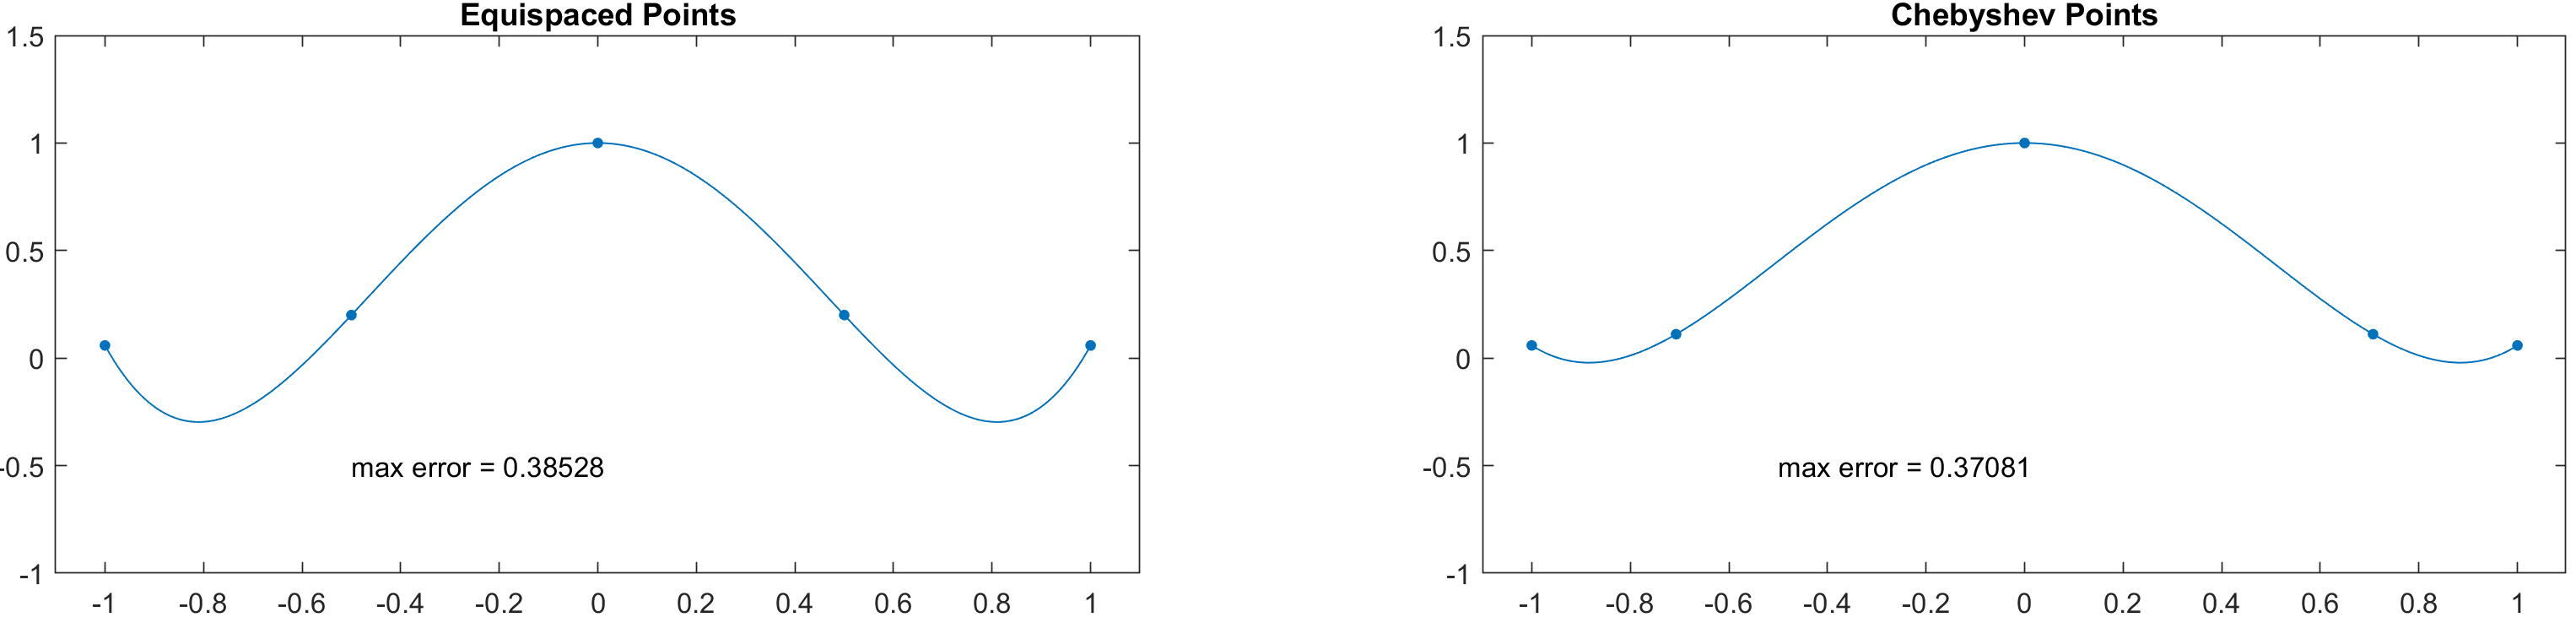
\includegraphics[scale=0.2]{5_14.PNG}
        \caption{$N=4$}
    \end{figure}
    \begin{figure}[htp]
        \centering
        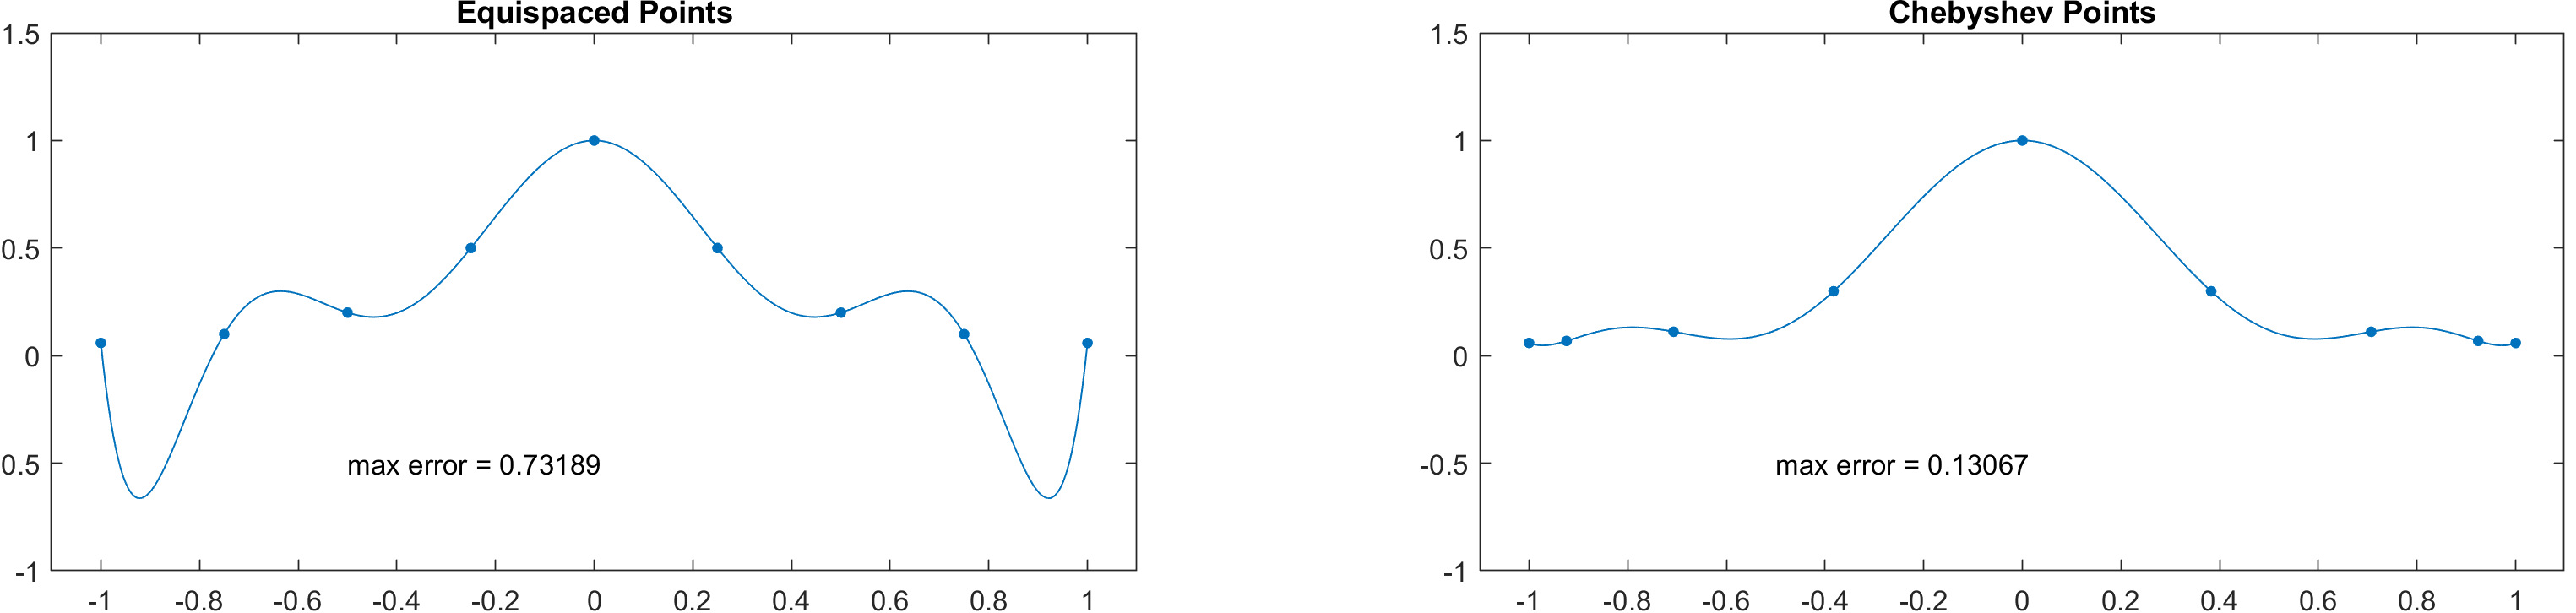
\includegraphics[scale=0.2]{5_18.PNG}
        \caption{$N=8$}
    \end{figure}
    \begin{figure}[htp]
        \centering
        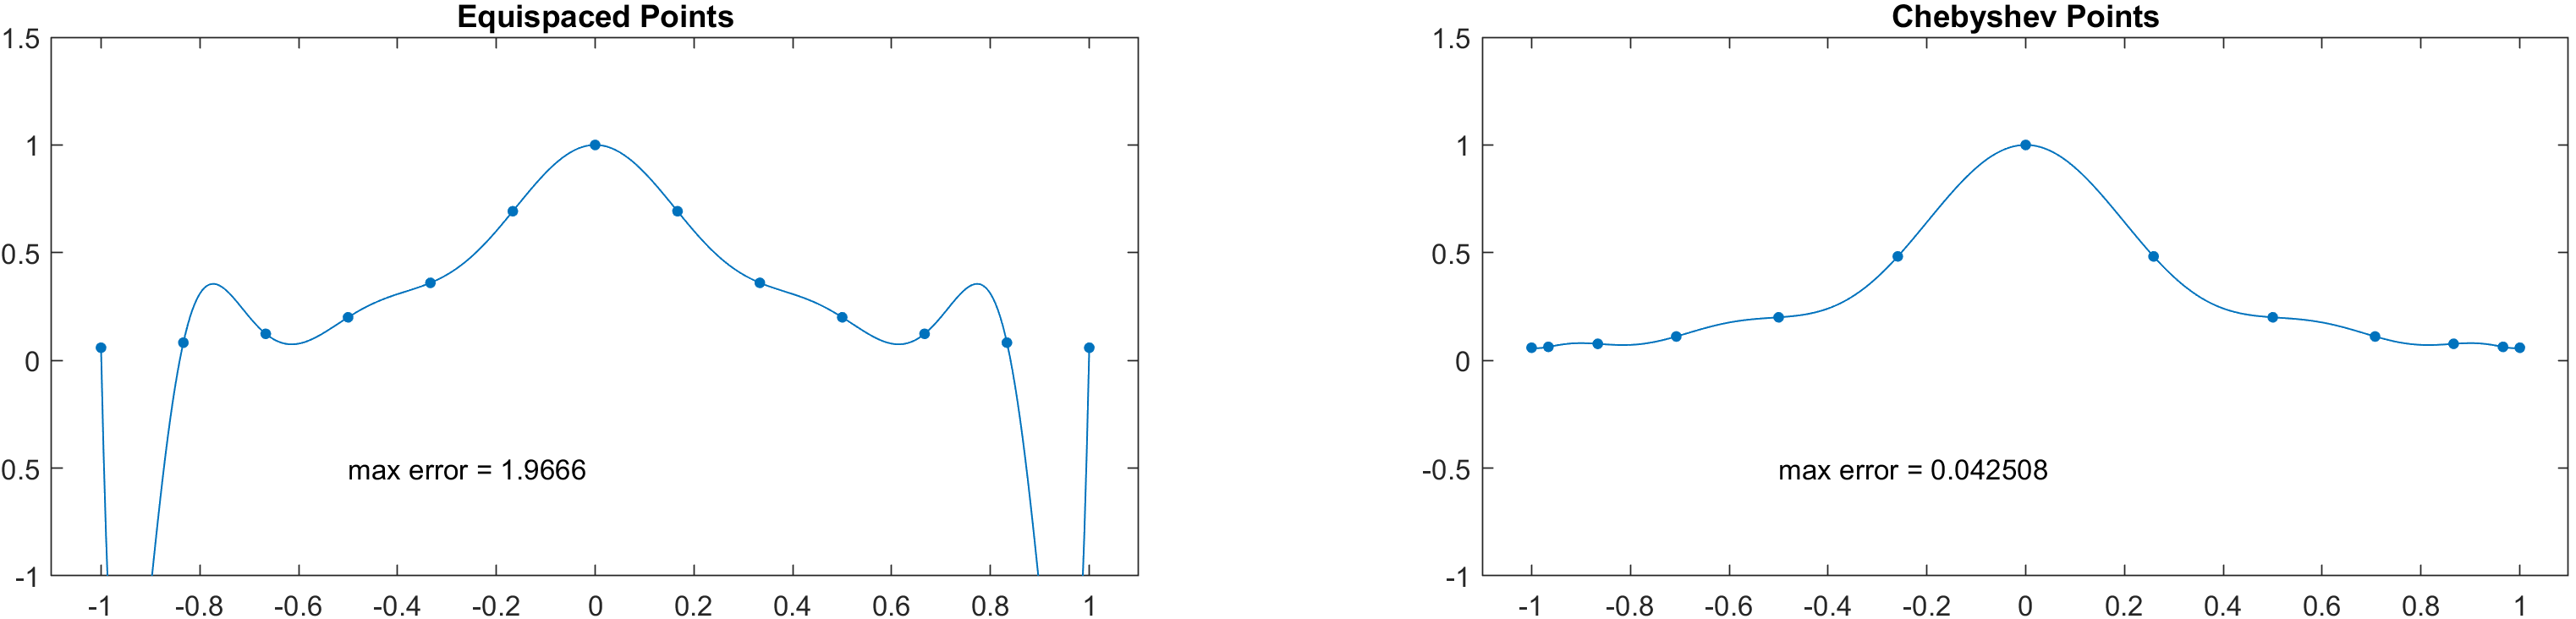
\includegraphics[scale=0.2]{5_112.PNG}
        \caption{$N=12$}
    \end{figure}
    \begin{figure}[htp]
        \centering
        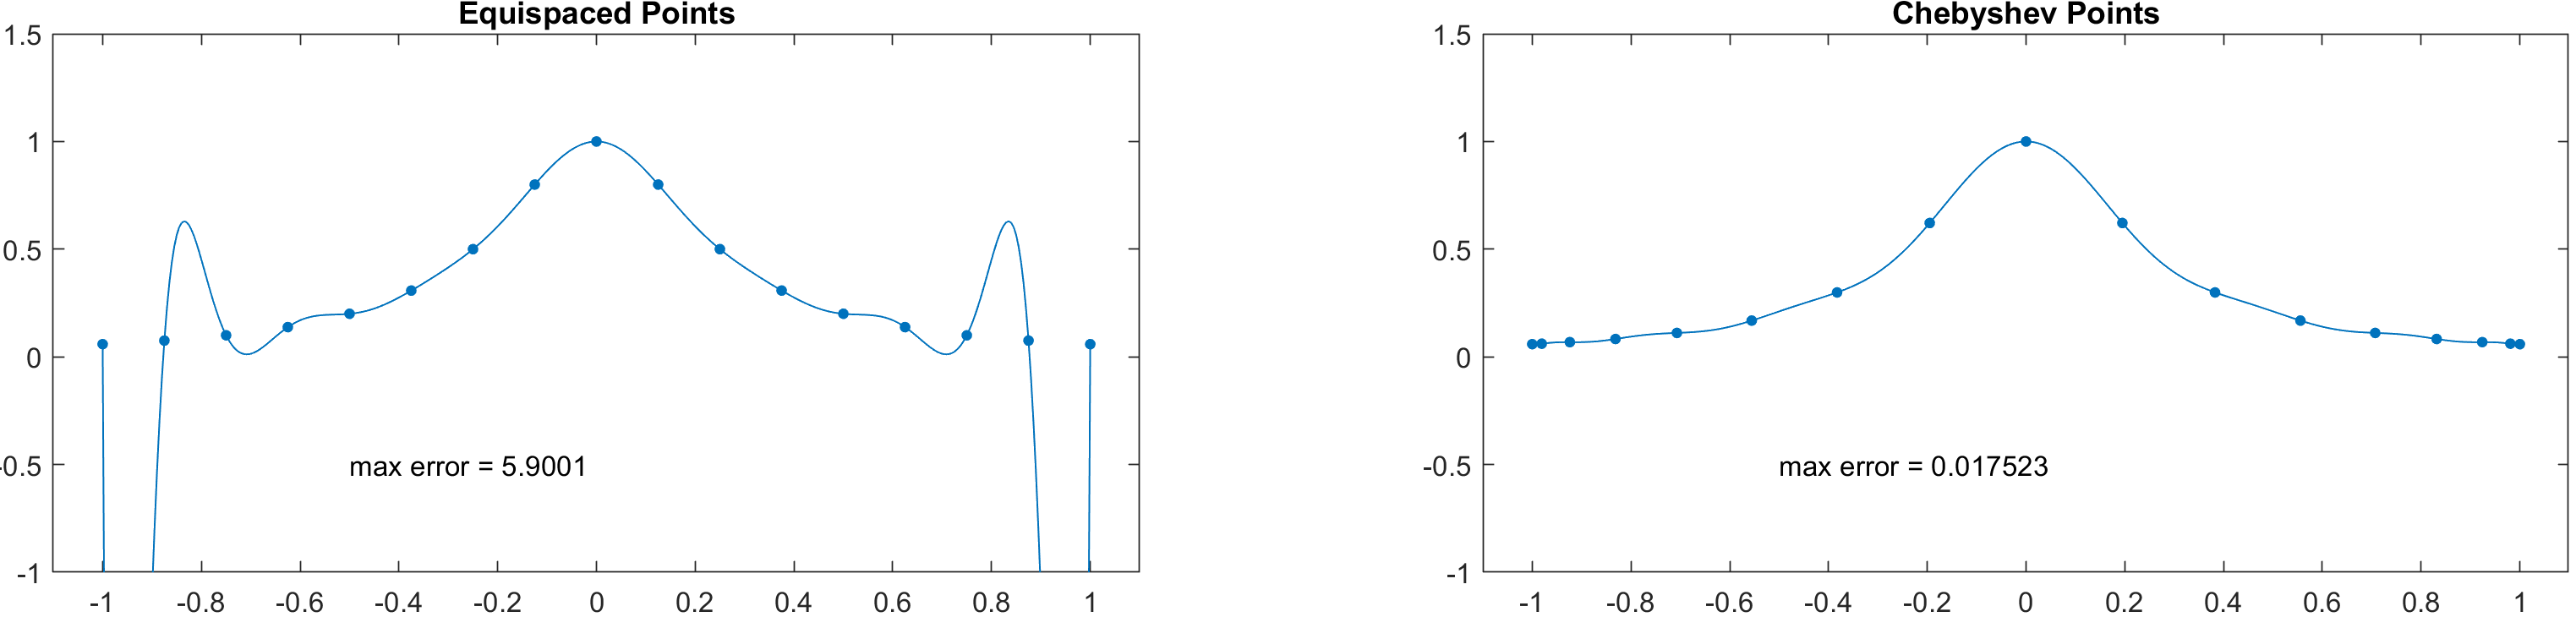
\includegraphics[scale=0.2]{5_116.PNG}
        \caption{$N=16$}
    \end{figure}
    \begin{figure}[htp]
        \centering
        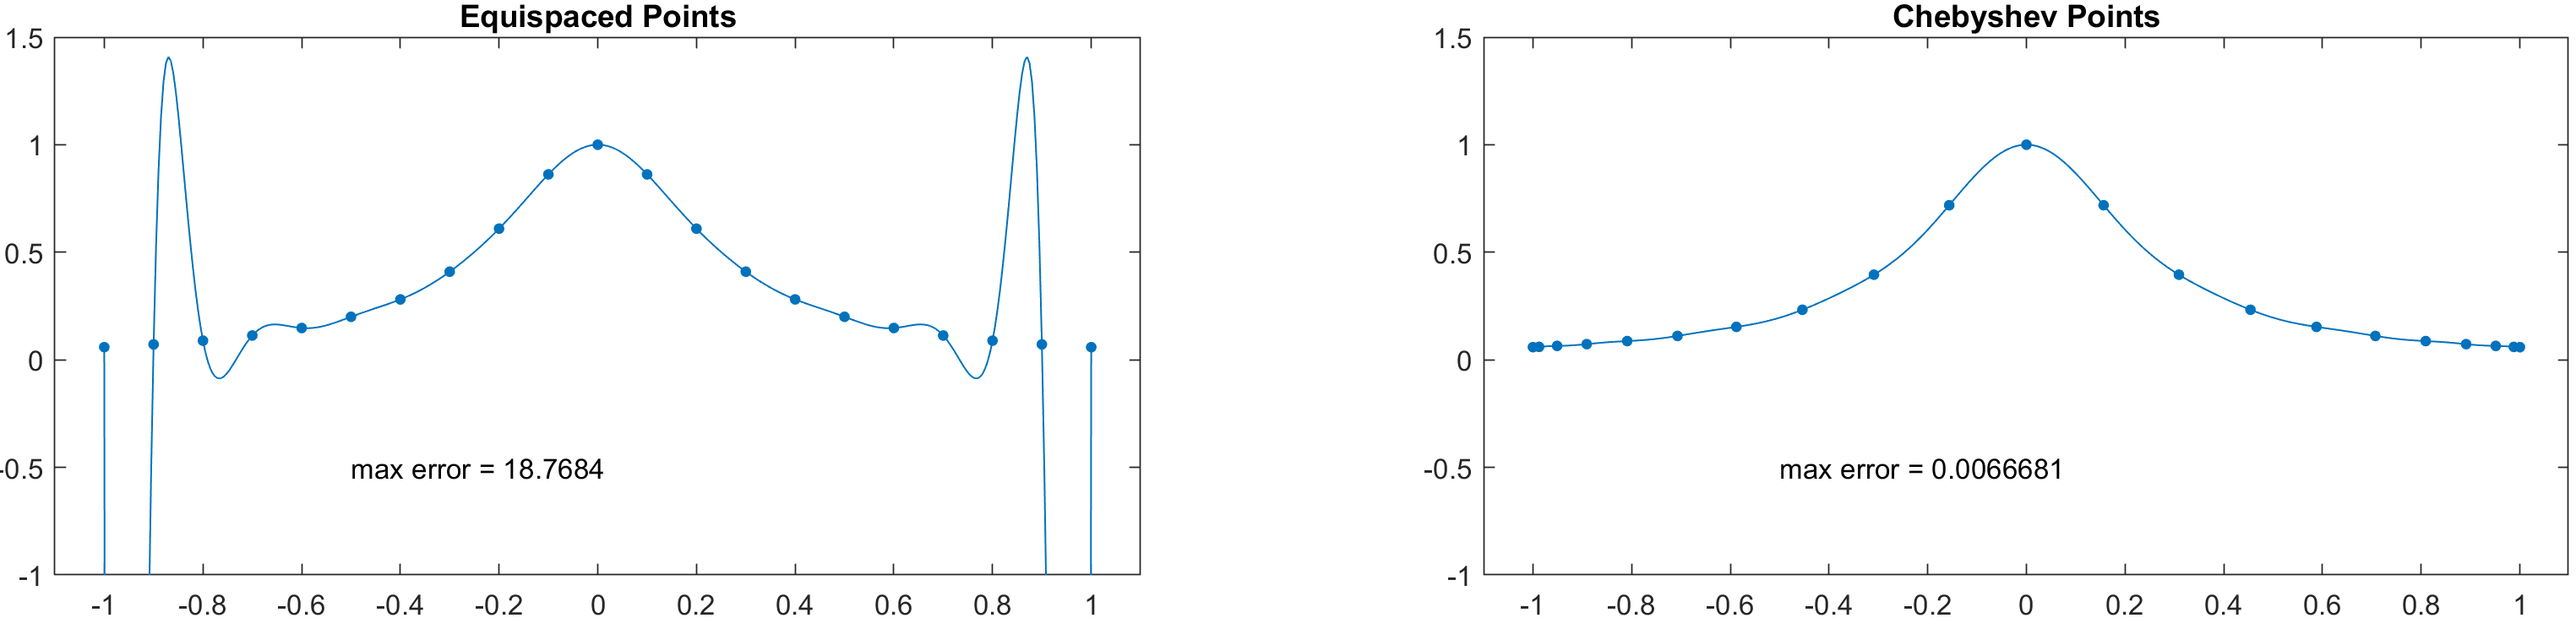
\includegraphics[scale=0.2]{5_120.PNG}
        \caption{$N=20$}
    \end{figure}
    \begin{figure}[htp]
        \centering
        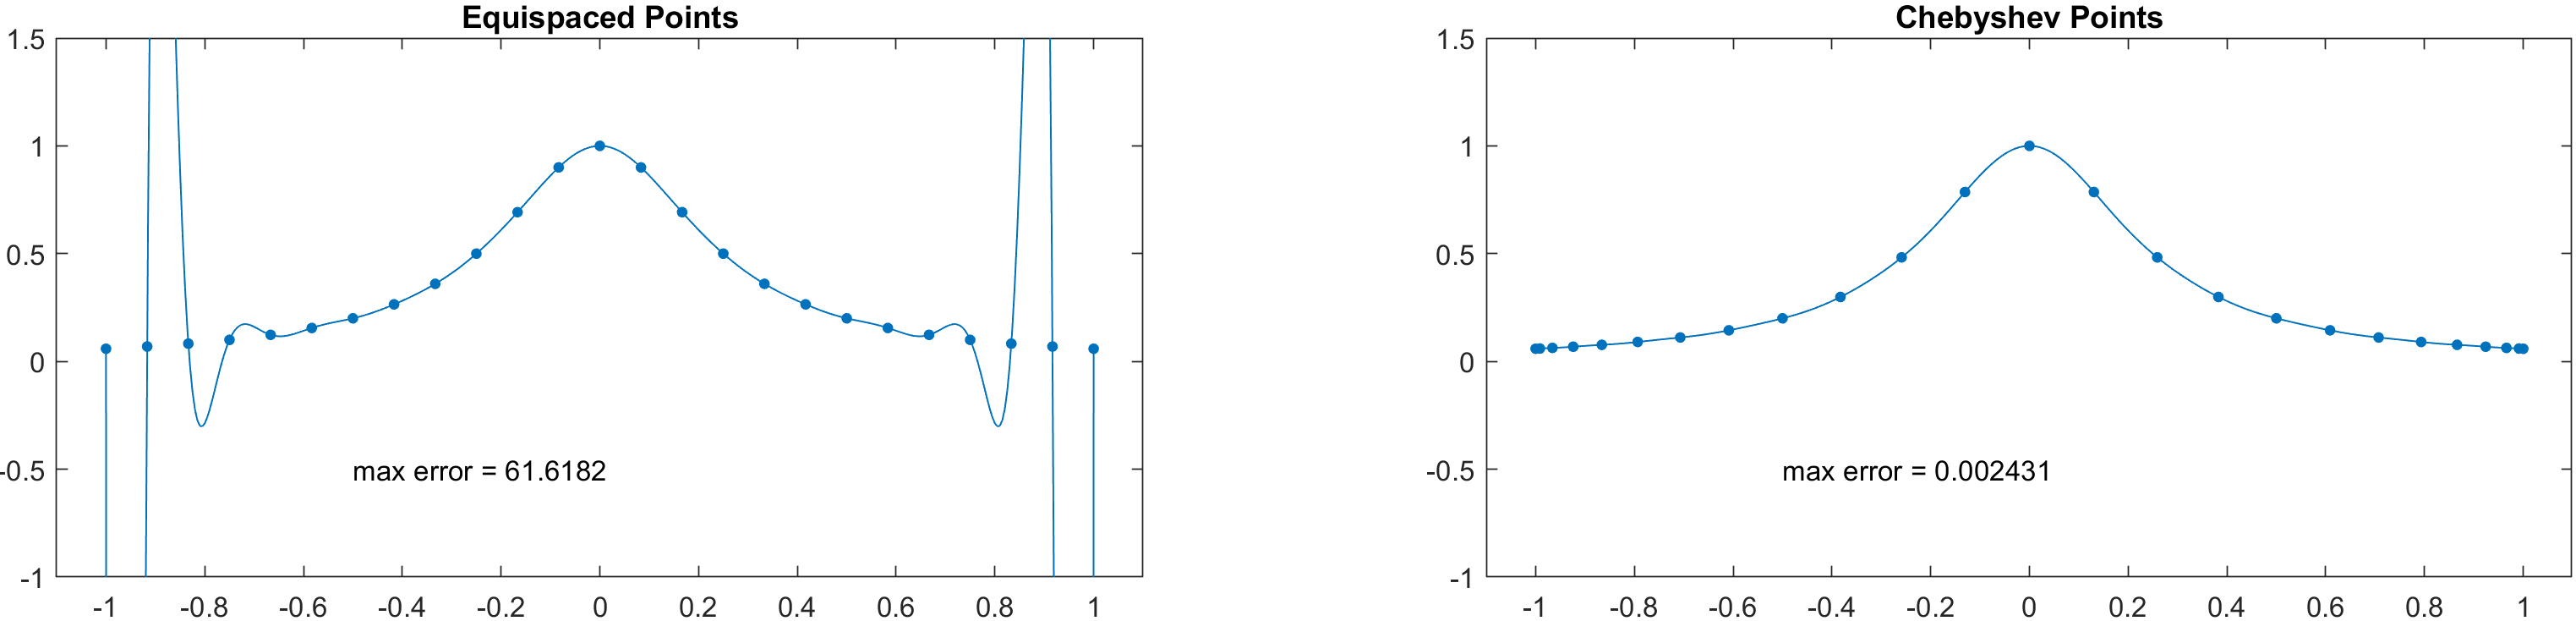
\includegraphics[scale=0.2]{5_124.PNG}
        \caption{$N=24$}
    \end{figure}
    \begin{figure}[htp]
        \centering
        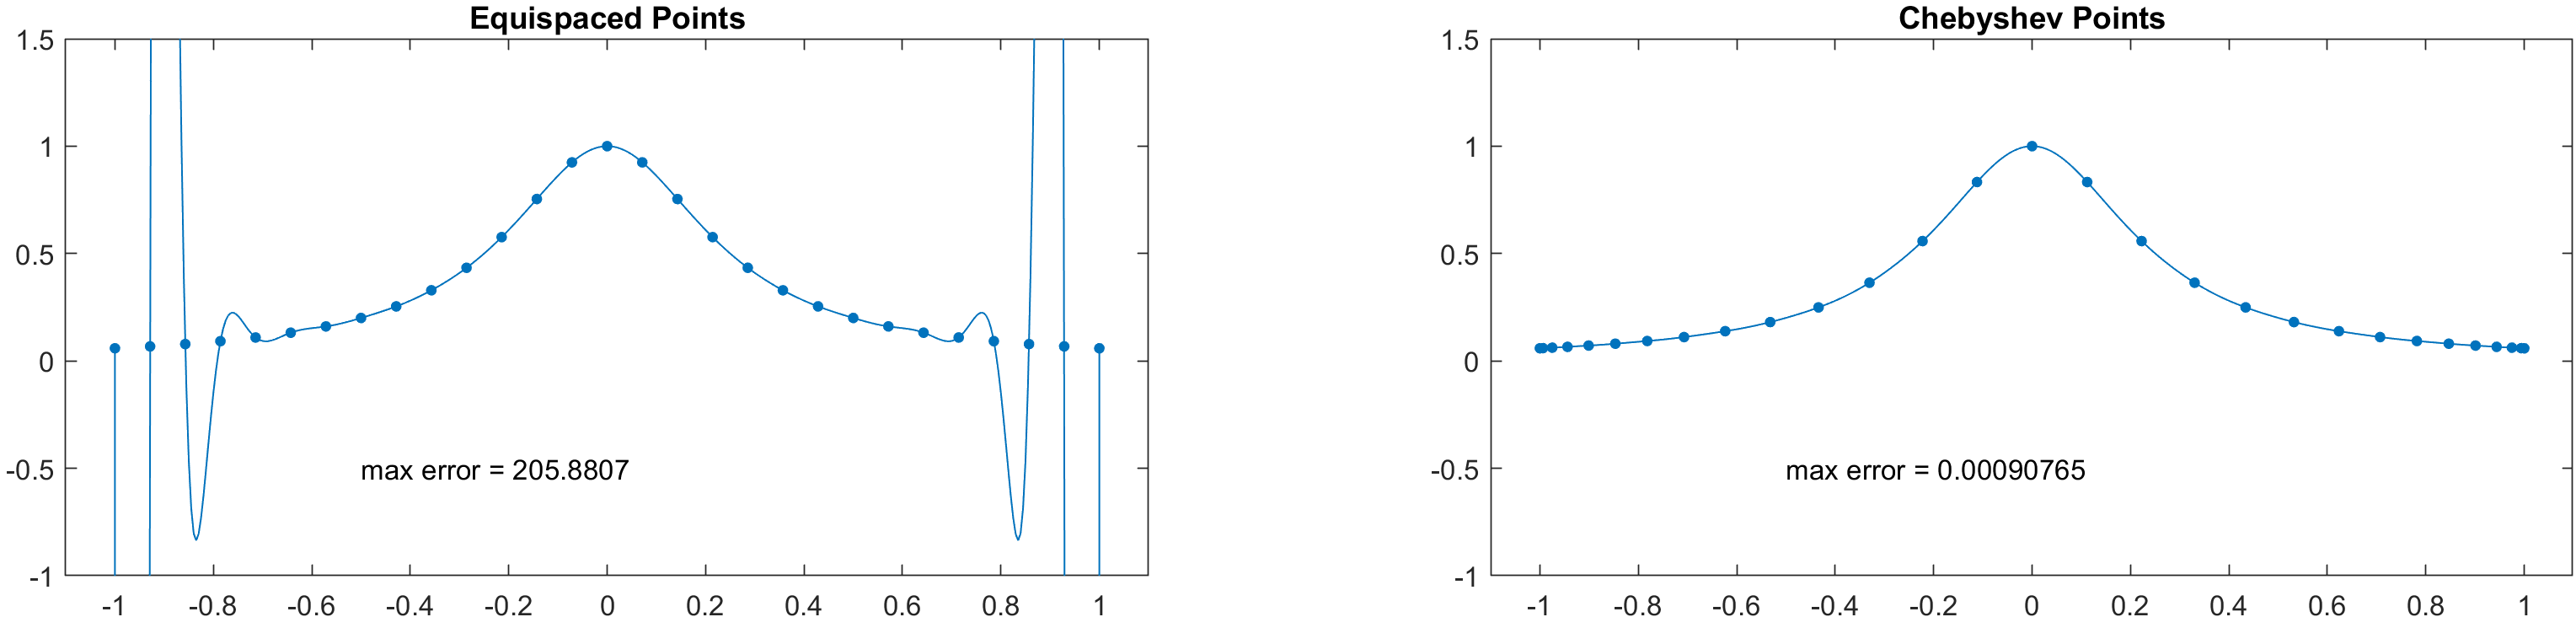
\includegraphics[scale=0.2]{5_128.PNG}
        \caption{$N=28$}
    \end{figure}

    Now, looking at the two plots of the error vs $N$, we see that for the equidistal points, there is no convergence.
    Rather, there is divergence towards infinity and this divergence happens exponentialy. Similarly, for the Chebyshev
    nodes, there is an exponential plotting, however, this is exponentially convergent.\\

    \begin{figure}[htp]
        \centering
        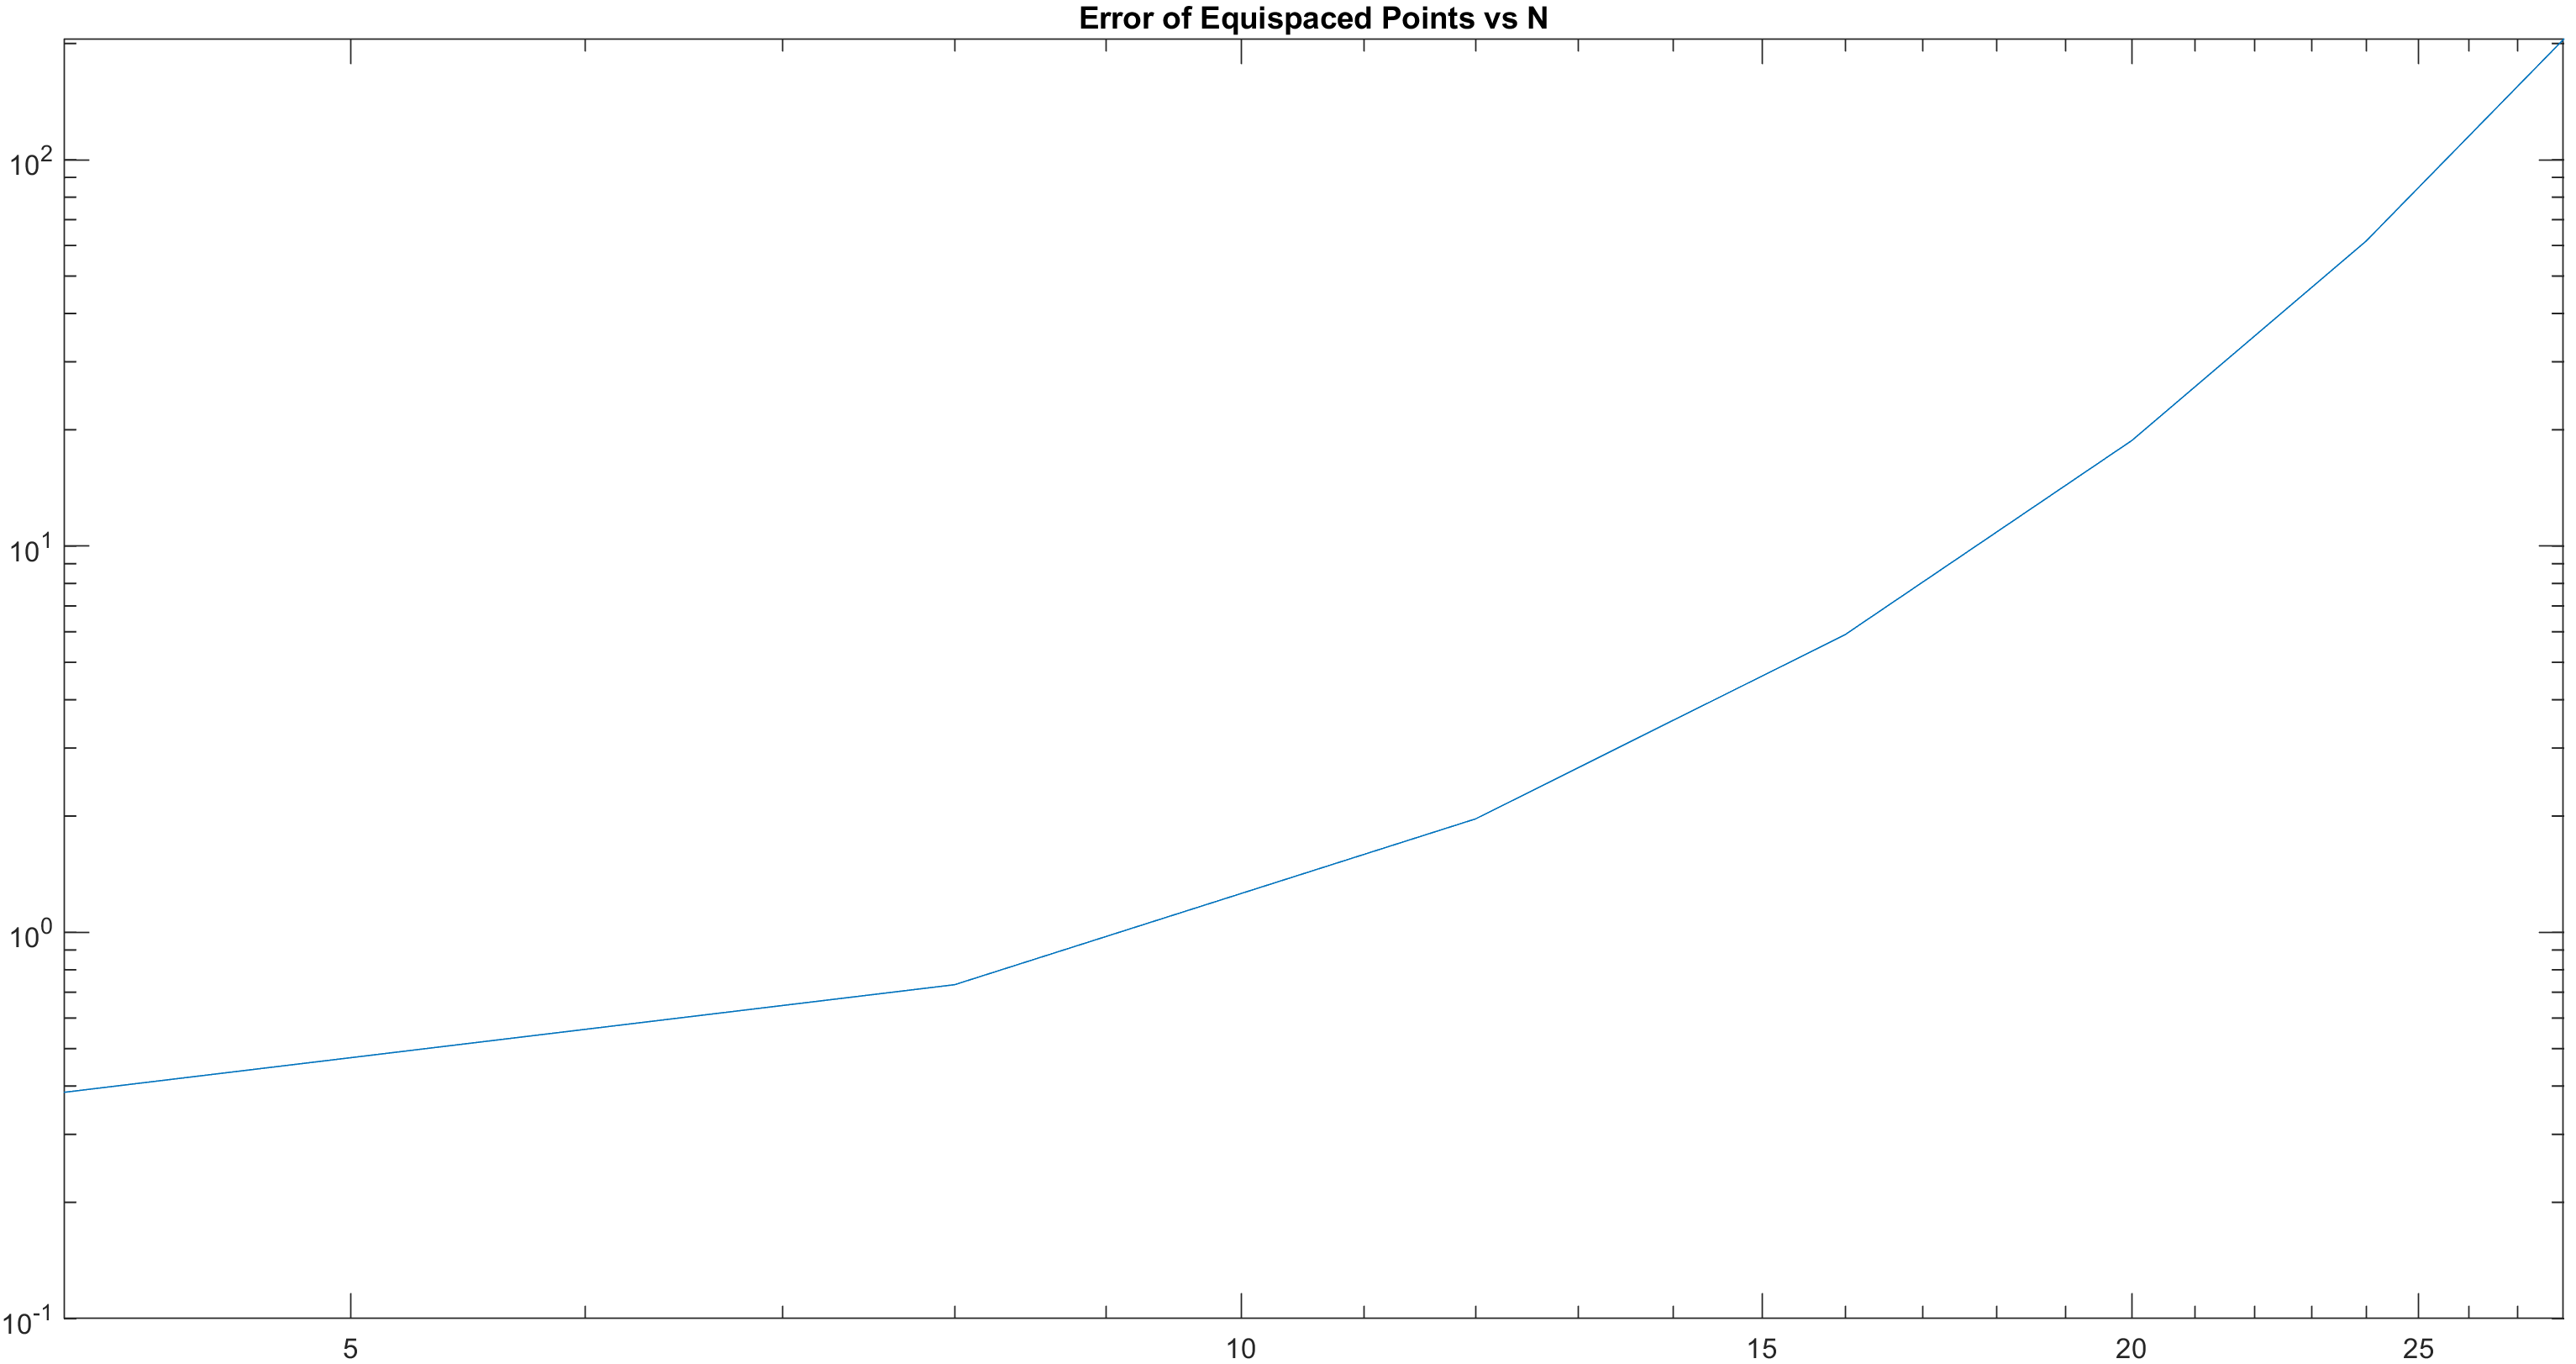
\includegraphics[scale=0.12]{5_1equi.PNG}
    \end{figure}
    \begin{figure}[htp]
        \centering
        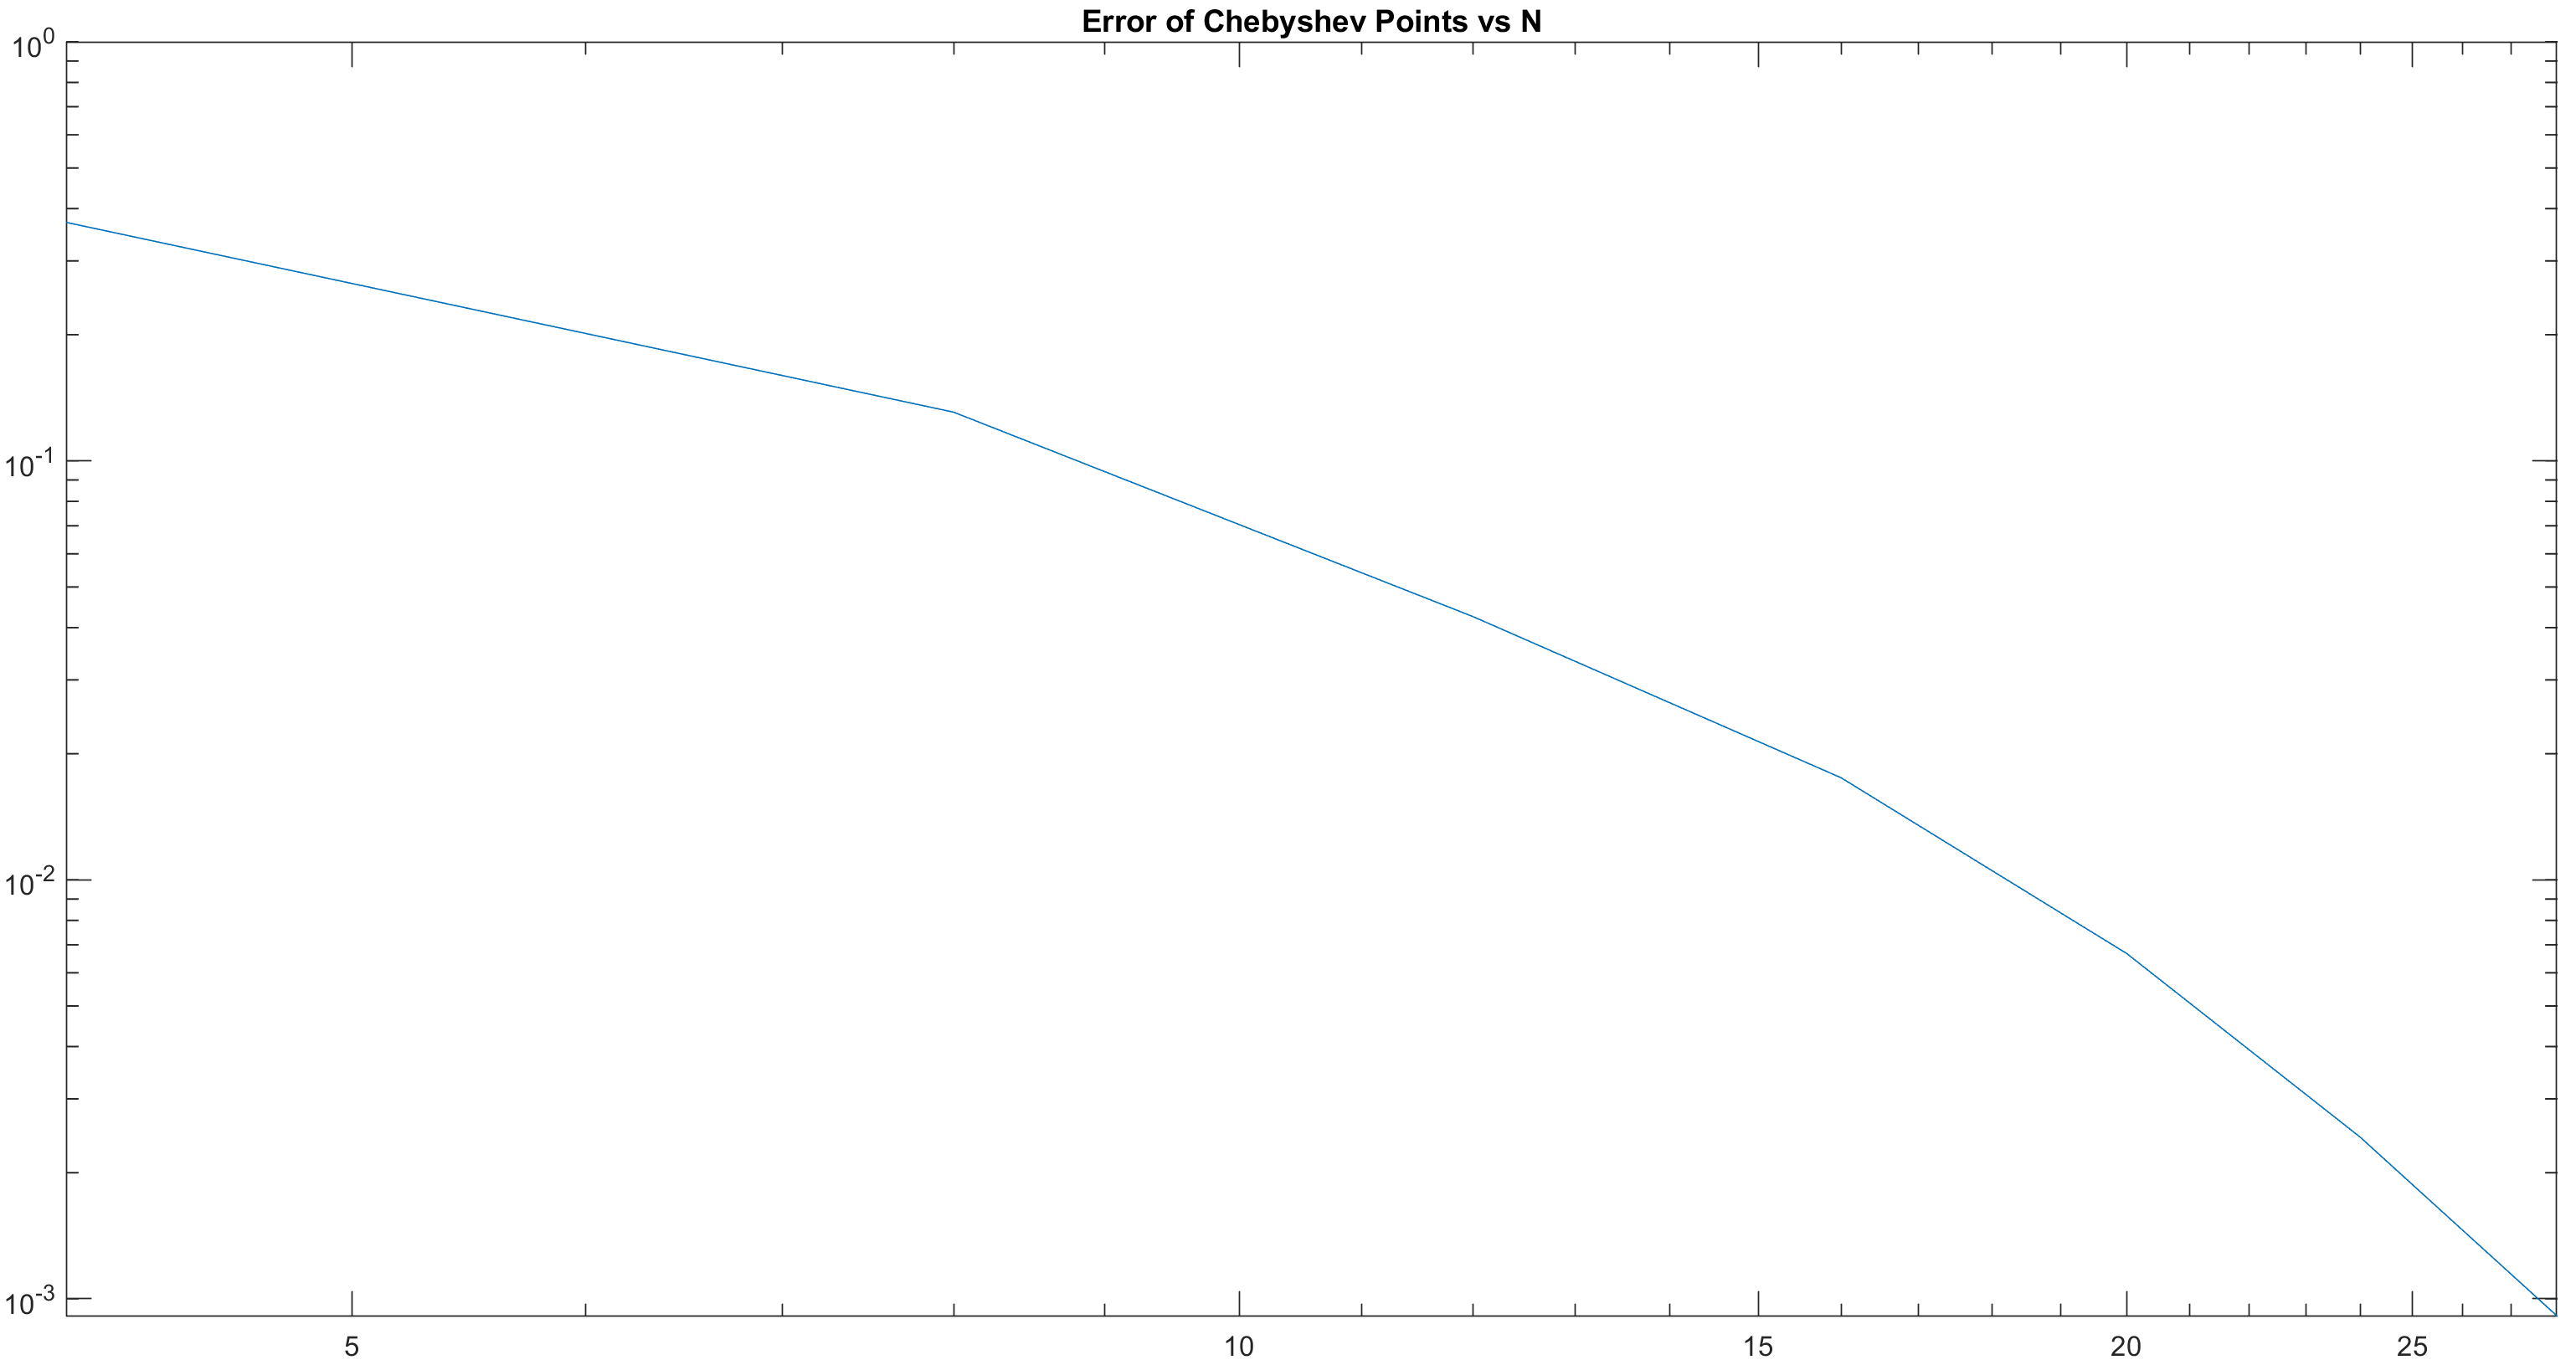
\includegraphics[scale=0.12]{5_1cheb.PNG}\\
    \end{figure}

\end{solution}

\newpage
\lstinputlisting{problem5_1.m}
\newpage